\chapter{研究方法}
\label{章:研究方法}

\section{漢羅全羅對齊}
\label{節:漢羅全羅對齊}
佇\ref{節:數位典藏}節有講著,數位典藏是提供漢羅佮全羅的對照,因為咱的翻譯需要一个漢字對一个音標的一對一,所以愛共數位典藏伊原本一段對齊一段的語料改做一字對一字。
而且愛注意數位典藏佇2006年完成,教育部的漢字規範對2007年才公佈,所以⿰因兩个的用字規範嘛是無仝款的。
毋過數位典藏的語料倩人整理的時陣內部有訂標準,伊的漢字有一半以上攏是會用得的,而且本論文以教育部的為主,所以
對齊的做法是共全羅逐字攏去對看覓漢羅,看佗一个組合會佇字典內底

%有1個少年人;伊抵tng7 teh 想
%U7 chit8 e5 siau3-lian5 lang5; i tu2-tng7 teh siuN7 phok-su7 lun7-bun5, 



\section{改變語料格式}
\label{節:改變語料格式}

\begin{figure}
\centerline{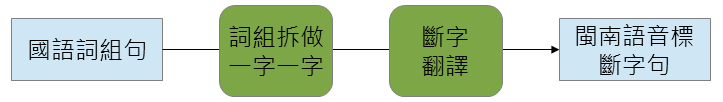
\includegraphics[keepaspectratio,width=40em]{圖/改變語料格式}}
\caption{改變語料格式流程}
\label{改變語料格式}
\end{figure}

頂一節發覺若用詞組當做翻譯的單位,會因為詞組單位傷大,變做真濟詞組無看過。
所以咱都共照圖\ref{改變語料格式}華語佮閩南語攏用一字一字做翻譯的單位,
共原本的「陸續 開放 一百五十項 的 規費」,變做「陸 續 開 放 一 百 五 十 項 的 規 費」。
照按呢共訓練語料變做一字一字,共這句翻譯會當得著「陸|liok8 續|siok8 開|khai1 放|hong3 一|tsit8 百|pah4 五|goo7 十|tsap8 項|hang7 的|e5 規|kui1 費|hui3 ,|,」,
效果比原本斷詞組的閣較好,得著82.94分。

語料格式的影響著翻譯的效果,除了斷字,翻譯嘛會使用斷詞做單位,華語用中研院中文斷詞系統(CKIP)\footnote{\url{http://ckipsvr.iis.sinica.edu.tw/}}斷詞,閩南語用辭典斷詞\footnote{實際按怎做請看\ref{節:拄好長度斷詞}}。「」提去翻譯會得著「」。斷詞的分數是76.88分,比斷詞組閣較好一寡,毋過小較輸斷字。三个分數整理佇表\ref{表:斷詞組、斷詞、斷字做單位的翻譯分數}。

\begin{table}
\caption{斷字、斷詞佮斷詞組做單位的分數}%
\label{表:斷詞組、斷詞、斷字做單位的翻譯分數}
\centering
\begin{tabular}{c|ccc}
翻譯單位 & 斷字 & 斷詞 & 斷詞組\\
\hline
分數 & 82.94 & 76.88 & 70.67\\
\end{tabular}
\end{table}

\section{拄好長度斷詞}
\label{節:拄好長度斷詞}
新聞語料庫是斷詞組,為著翻譯的效果需要改做斷詞,啊拄好教育部辭典佮數位典藏有全羅標記斷詞的狀況,就會使提來幫助新聞語料庫斷詞。

斷詞的標準有誠濟種,為著方便,以教育部的「臺灣閩南語羅馬字拼音方案連字符使用原則」的連字符當做一个詞,若「tsiah8 png7」(食白米飯的意思),當做兩个詞,「tsiah8-png7」(食物件的意思),當做一个詞。

定看著的斷詞方法有上長詞優先\footnote{(FMM)},伊的做法是自頭開始,看頭前幾个字是毋是會當揣著一个佇辭典的詞,若會使,就揀上長的彼个,…%解釋比如說,『我想要吃飯』可以切成『我,想,要,吃,飯』『我,想要,吃飯』『我,想要吃飯』『我想要,吃飯』『我想要吃飯』,其中,能夠在字典找到詞的切割方式有『我,想,要,吃,飯』『我,想要,吃飯』,
%ㄍㄛˊ
因為上長詞有時陣會揀著無好的組合,親像「」「」
%j揣一个1+3比2+2較歹的例
為著閃避這種情形,莫予長詞搶短詞的字,咱就用「拄好長度斷詞」。斷詞的方法是佮上長詞優先相像,詞仝款愈長愈好,毋過咱予無仝長度的詞無仝分數,設定上長四字詞,一字詞1分、兩字詞1/2分、三字詞1/3分、四字詞1/4分,閣用維特比(Viterbi)揣分數上低的斷詞切法。親像「頭前 有 一張 椅仔」就是1/2+1+1/2+1/2=3分,若「」%用面頂2+2的例

毋過輸入的資料若是全羅「hoo7 i1 tsut4-khi3 sng2」,上好的答案是「hoo7 i1 tsut4-khi3 sng2/予伊出去耍」,但是拄好長度的斷詞煞會斷出「hoo7-i1 tsut4-khi3 sng2/雨衣出去耍」,這个情形上長詞優先嘛會拄著。毋過若有提供漢字,就袂拄著這種情形。

新聞語料庫的華語部份用中研院中文斷詞系統(CKIP)\footnote{\url{http://ckipsvr.iis.sinica.edu.tw/}}斷詞

\section{未知詞另外翻譯}
\label{節:未知詞另外翻譯}

\begin{figure}
\centerline{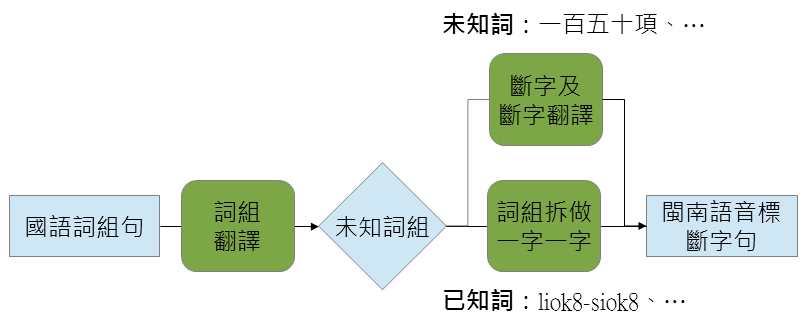
\includegraphics[keepaspectratio,width=40em]{圖/未知詞另外翻譯}}
\caption{未知詞另外翻譯流程}
\label{未知詞另外翻譯}
\end{figure}

對頂頭的結果來看,用斷字來做翻譯較袂拄著未知詞的問題。換別的角度來看,準若咱用斷詞組的翻譯模型,拄著未知詞的時陣,這个未知詞會使提予斷字翻譯模型去翻譯,就是講「陸續 開放 一百五十項 的 規費」提予斷詞組模型翻譯,得著「liok8-siok8 khai1-hong3 一百五十項 e5 規費」,閣來共「一百五十項」佮「規費」這兩个詞組切做斷字「一 百 五 十 項」佮「規 費」,閣擲去斷字模型翻譯,流程會當看圖\ref{未知詞另外翻譯},按呢得著84.85分。

毋過按呢閣無夠,\ref{節:改變語料格式}節的結果證明仝一份語料無仝形式會有無仝的結果,所以閣愛看覓佇斷詞、斷字的情形之下,翻譯效果是按怎變化的。

咱做的是華語翻譯到閩南語,攏總兩个語言,逐个語言有斷詞組、斷詞佮斷字三種方法,實驗都有$3^{2}=9$組合,分數請看表\ref{表:華語閩南語逐種形式,而且未知詞提予斷字模型翻譯的結果}。
全部分數上懸的是華語斷詞組對閩南語斷詞組,原因是伊斷的詞組,對訓練翻譯模型需要對齊模型的語詞對照表\footnote{若袂記得,請看\ref{節:翻譯架構}節的說明}有幫助。
而且毋管閩南語的狀態,華語斷詞攏比華語斷字閣較好,因為中研院中文斷詞系統會共定定用的詞組當作詞,親像「看 書」因為是定用詞組,會合做伙做「看書」,看無遐爾用著的「看 電視」猶原是「看 電視」。

毋過閩南語斷字變斷詞了後,效果煞較\ji{⿰禾黑},是因為閩南語斷詞干焦用辭典\footnote{實際按怎做請看\ref{節:拄好長度斷詞}}爾爾,而且詳細去比較「華語斷詞-閩南語斷字」佮「華語斷詞-閩南語斷詞」的結果,6954句內底有1367句無仝,用人工看頭前151組無仝的結果,逐組揀1个較好的。有71組是斷字的結果較好,有56組是斷詞模型較好,賰的24組是口腔無仝,當做是平平仔好。
閣去查斷詞為啥物翻譯較\ji{⿰禾黑},詳細看原本斷詞的內容,「遊|iu5 客-人|kheh4-lang5 數|soo3」斷做「遊|iu5 客-人|kheh4-lang5 數|soo3」,都有淡薄仔問題矣,才會拖著翻譯效果。
%會使講準做「華語斷詞-閩南語斷字」的分數比「華語斷詞-閩南語斷詞」較懸,毋過人來看,煞無一定是按呢。

\section{漢羅全羅轉一對一}
\label{節:漢羅全羅轉一對一}
共漢羅全羅一字一字對齊了後,會發覺一个問題,有的字是一對一,有的字煞干焦音標爾。
翻譯格式一致會予效果閣較好,所以就愛共干焦音標的漢字補起來變一對一。頭一步就是用\ref{節:拄好長度斷詞}節的方法來斷詞,因為有的詞可能一字一對一、一字音標,親像「彰化」,寫做「tsiong1化」,按呢佇辭典內底加逐種可能,閣愛加「彰hua3」、「彰tsiong1 hua3」、…攏總九種\footnote{漢字、音標、一對一三種兩字,攏總$3^{2}=9$種}。為著查字典的速度閣較緊,就親像圖XX仝款,逐个詞一字一字處理落來,逐字分做漢字、音標、一對一三个點,第二个字閣佇這三个點閣生落去,毋過第一个字有佮別的詞仝款,就會使公家一个點,親像「彰化」「將來」「將軍庄」,因為限制上長四字詞\footnote{照教育部的「臺灣閩南語羅馬字拼音方案連字符使用原則」,有可能有五字詞,毋過這擺實驗限制四字詞},一个詞上濟產生120點\footnote{第一層加到第四層,$3^{1}+3^{2}+3^{3}+3^{4}=120$},毋過揣候選詞的時間複雜度是$O(1)$。

決定斷詞斷佇佗位了後,逐个斷詞的所在可能有超過一个的候選詞,「彰化的米誠好食」,
上尾閣用語言模型,配合維特比算法,揀出機率上懸的詞組。


\begin{table}
\caption{華語閩南語逐種形式,而且未知詞提予斷字模型翻譯的結果}%
\label{表:華語閩南語逐種形式,而且未知詞提予斷字模型翻譯的結果}
\centering
\begin{tabular}{c|ccc}
\diaghead{\theadfont Diag ColumnmnHead II}%
{華語形式}{閩南語形式} & 斷字 & 斷詞 & 斷詞組\\
\hline
斷字 & 82.94 & 82.75 & 80.61\\
斷詞 & 84.27 & 84.05 & 82.89\\
斷詞組 & 84.05 & 83.90 & 84.85\\
\end{tabular}
\end{table}


\section{語言判斷特徵}
\label{節:語言判斷特徵}
為著予電腦會當分別閩南語佮華語,咱就愛準備幾項閩南語佮華語無仝的特徵。
閩南語佮華語上大差別就是用詞無仝,閩南語寫「食飯」、「無法度」,華語寫「吃飯」、「沒辦法」,
所以咱揀定用詞出來,當作咱的特徵之一。
毋過閩南語佮華語有誠濟共同詞,親像「火車」、「電腦」,⿰因寫法是仝款的,所以咱袂使直接提定用詞來做,因為內底會有共同詞,所以咱愛對閩南語定用詞內底揀華語袂用的特徵詞出來,華語嘛仝款愛揀出閩南語袂用的特徵詞。

選特徵詞的方法是先統計\ref{節:整理實驗流程佮結果}的試驗語料佮數位典藏,揀出頭前15000个上定出現的閩南語定用詞\footnote{有標點符號}
華語部份嘛仝款,佇中央研究院現代漢語標記語料庫\footnote{\url{http://app.sinica.edu.tw/cgi-bin/kiwi/mkiwi/kiwi.sh}}內底揣15000个上定出現的華語定用詞,
閣來對上定用的閩南語定用詞開始,若這个定用詞的漢字詞無出現佇華語15000定用詞內底,就共伊當做特徵詞。
若伊出現佇華語定用詞內底,就莫治。
就按呢揀出頭前7000个特徵詞。
華語的部份嘛仝款,揀出7000个無佇閩南語定用詞的特徵詞。

%看圖

有閩南語佮華語的特徵詞了後,咱對網頁整理出一段一段的語料,先用\ref{節:拄好長度斷詞}節的閩南語斷詞,看斷詞出來的結果,佇閩南語7000个特徵出中,分別出現幾个。
除了7000个特徵詞,咱閣用閩南語語言模型分數,斷詞了的全部詞數,1~4字詞分別數量\footnote{「我 想 欲 食飯」就有3个一字詞,1个兩字詞,全部4个詞},按呢干焦閩南語就有7006个特徵,摻華語就有14012个特徵。


頂一節決定特徵了後,紲落來就是愛決定辨識的模型,親條圖\ref{圖:判斷語言架構}。
逐个辨識模型效果佮用途無仝,揀效果較好的幾个來實驗。

\begin{figure}
\centerline{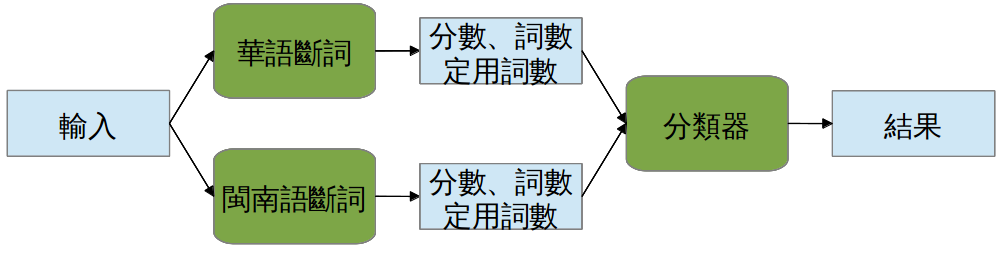
\includegraphics[keepaspectratio]{圖/判斷語言架構}}
\caption{判斷語言流程}
\label{圖:判斷語言架構}
\end{figure}


頂一章使用新聞語料庫,語言模型嘛是用平行語料的閩南語訓練的,其實這馬有一大部份的閩南語語料攏毋是平行話料,攏是純閩南語一種語言爾爾。
這種純閩南語的語料其實嘛會當提來訓練語言模型,毋過語料的形式就有足濟款的,親像有漢羅、全羅佮全漢等等。有的語料會敆兩種以上的文本。
毋過語料的形式無仝,會當利用的部份就無仝。親像全羅會當提供斷詞的資訊,有漢字佮拼音一對一的當提來做辭典。
這章會加入新的語料庫,而且利用⿰因無仝款的性質,親像圖\ref{圖:互相整理架構}來互相整理,翻譯的效果閣較好。

\begin{figure}
\centerline{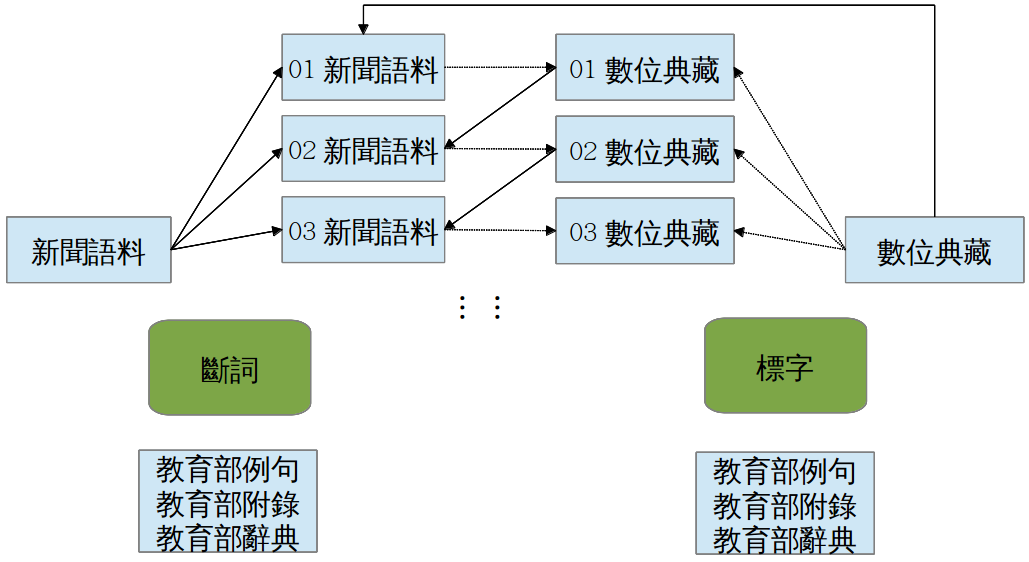
\includegraphics[keepaspectratio,width=40em]{圖/互相整理架構}}
\caption{互相整理流程}
\label{圖:互相整理架構}
\end{figure}




